\documentclass[slidestop,xcolor=pst,dvips,blue]{beamer}

\usepackage{beamerthemesplit}
\usepackage[utf8]{inputenc}
\usepackage[spanish]{babel}
\usepackage{graphicx}
\usepackage{pstricks} % PSTricks package
\usepackage{setspace}
\usepackage{multirow}
\usepackage{listings}
\usepackage{pgfpages}
\usepackage{hyperref}
\usepackage{etoolbox}
\usepackage{epstopdf}

\makeatletter
\patchcmd{\beamer@sectionintoc}{\vskip1.5em}{\vskip0.5em}{}{}
\makeatother

\setbeamercovered{dynamic}
\setcounter{tocdepth}{2}
\setbeamercolor{frametitle}{fg=black,bg=white}
\setbeamercolor{section in toc shaded}{fg=black}
\setbeamercolor{section in toc}{fg=red}
\setbeamercolor{subsection in toc shaded}{fg=black}
\setbeamercolor{subsection in toc}{fg=red}
\setbeamerfont{section in toc}{size=\small}
\setbeamerfont{subsection in toc}{size=\small}
\setbeamertemplate{section in toc shaded}[default][99]
\setbeamertemplate{subsection in toc shaded}[default][99]

\AtBeginSection[]
{\begin{frame}[c]
  \frametitle{Índice}
	\tableofcontents[currentsection,
        sectionstyle=show/shaded,
        subsectionstyle=hide]
\end{frame}}

\AtBeginSubsection[]
{\begin{frame}[c]
	\frametitle{Índice}
	\tableofcontents[
  		currentsection,
  		sectionstyle=shaded/shaded,
  		currentsubsection,
  		subsectionstyle=show/shaded/hide
		]
\end{frame}}

\setbeamercolor{frametitle}{fg=black,bg=white}

\setbeamertemplate{frametitle}{
	\begin{centering}
		\insertframetitle
		\par
	\end{centering}
}

\usetheme[secheader]{Boadilla} 

\newcommand{\imp}[1]{{\small{\sf #1}}}
\newcommand{\stk}{\emph{stakeholder}}

\title[Requisitos Funcionales]{Modelado y Especificación de Requisitos Funcionales}

\author[P. Sánchez]{\alert{Pablo Sánchez}}

\institute[IIE]{
		   Dpto. Ingeniería Informática y Electrónica \\
		   Universidad de Cantabria \\
		   Santander (Cantabria, España) \\
		   p.sanchez@unican.es
}

\date{}

\begin{document}

\begin{frame}[c]
	\titlepage
	\begin{columns}
		\column{0.50\linewidth}
			\centering
			
\includegraphics[width=.28\textwidth,keepaspectratio=true]{images/istr.eps}
		\column{0.50\linewidth}
			\centering
			
\includegraphics[width=.25\textwidth,keepaspectratio=true]{images/uc.eps}
    \end{columns}
\end{frame}

\begin{frame}[c]
    \frametitle{\alert{Advertencia}}
    \begin{center}
        Todo el material contenido en este documento no constituye en modo alguno una obra de referencia o apuntes oficiales mediante los cuales se puedan preparar correctamente las pruebas evaluables necesarias para superar la asignatura. \ \\
        \ \\
        Este documento contiene exclusivamente una serie de diapositivas cuyo objetivo es servir de complemento visual a las actividades realizadas en el aula.  \ \\
        \ \\
        Dicho de forma más clara, \alert{estas transparencias no son apuntes y su objetivo no es en modo alguno servir para que el alumno pueda preparar la asignatura.}
    \end{center}
\end{frame}

\begin{frame}[c]
    \frametitle{Objetivos del Tema}
    \begin{enumerate}[<+->]
         \item Entender el papel de los modelos orientados a solución en los Procesos de Ingeniería de Requisitos.
         \item Aprender a descomponer jerárquicamente requisitos, utilizando tanto objetivos como escenarios.
         \item Aprender a especificar requisitos de alto nivel utilizando objetivos.
         \item Aprender a especificar requisitos de nivel medio utilizando escenarios.
         \item Aprender a especificar requisitos de nivel medio utilizando historias de usuario.
         %% \item Aprender a priorizar requisitos.
    \end{enumerate}
\end{frame}

\begin{frame}[allowframebreaks,t]
    \frametitle{Bibliografía}
    \begin{thebibliography}{1}
\bibitem{lamsweerde:2009v2}
Axel van Lamsweerde.
\newblock {\em {Requirements Engineering: From System Goals to UML Models to
  Software Specifications}}.
\newblock Wiley, January 2009.

\bibitem{cockburn:2000v2}
Alistair Cockburn.
\newblock {\em {Writing Effective Use Cases}}.
\newblock Addison-Wesley, Octubre 2000.

\bibitem{pohl:2010v2}
Klaus Pohl.
\newblock {\em {Requirements Engineering: Fundamentals, Principles and
  Techniques}}.
\newblock Springer, June 2010.

\bibitem{itu:urnv2}
International Telecommunication Union (ITU).
\newblock {\em {User Requirements Notation (URN) \- Language Definition}}.
\newblock Standard Z.151. Octubre 2012.

\bibitem[Cohn, 2004]{Cohn2004}
Cohn, M. (2004).
\newblock {\em {User Stories Applied: For Agile Software Development}}.
\newblock Addison-Wesley Professional.
\end{thebibliography}
\end{frame}

\section{Introducción}

\begin{frame}
    \frametitle{Proceso de Ingeniería de Requisitos}
    \only<1>{
	\rput[lt](0,-0.5){
	   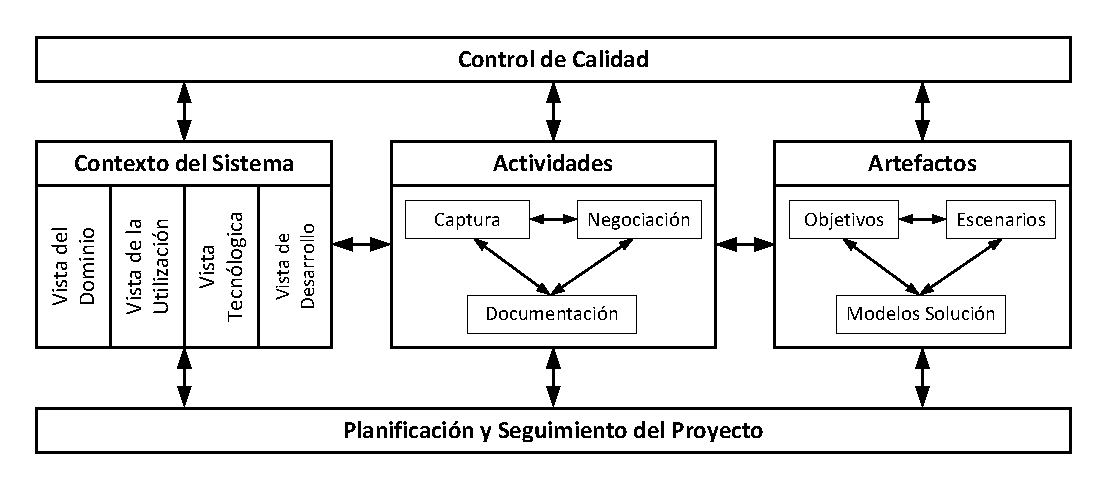
\includegraphics[width=11.5cm,keepaspectratio=true]{images/introduction/procesoIr00.eps}}
	}
    \only<2>{
	\rput[lt](0,-0.5){
	   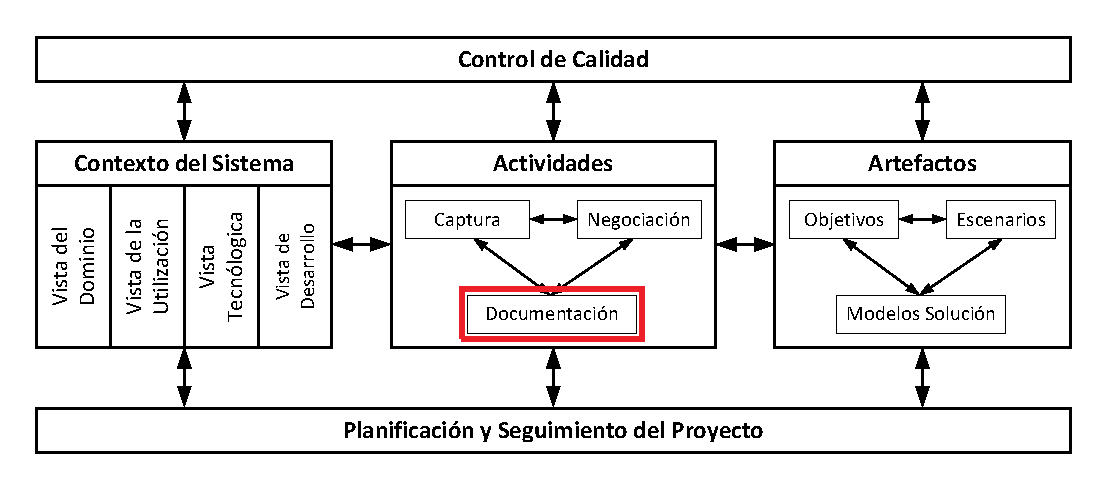
\includegraphics[width=11.5cm,keepaspectratio=true]{images/introduction/procesoIr01.eps}}
	}
    \only<3>{
	\rput[lt](0,-0.5){
	   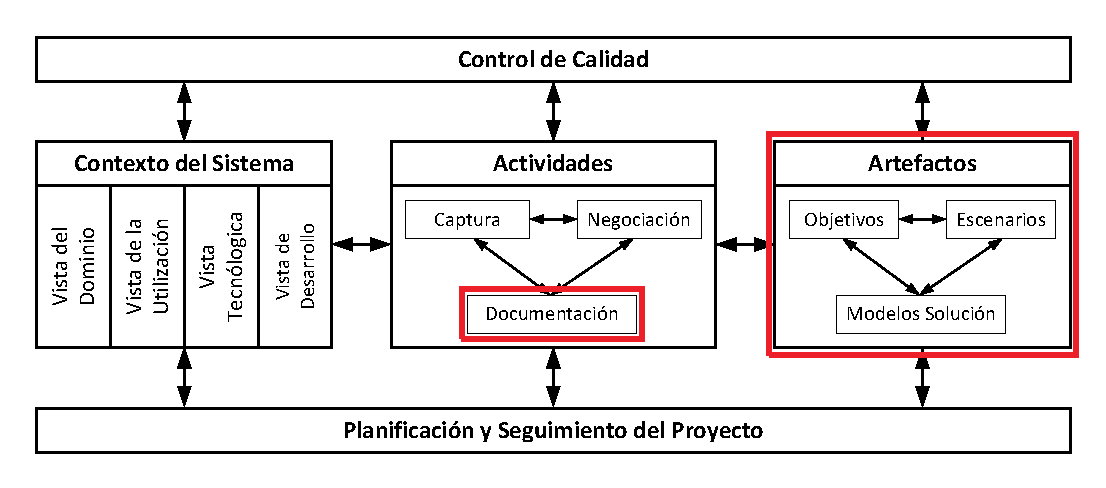
\includegraphics[width=11.5cm,keepaspectratio=true]{images/introduction/procesoIr02.eps}}
	}
\end{frame}

\section{Modelos Orientados a la Solución del Problema}

\begin{frame}
    \frametitle{Proceso de Ingeniería de Requisitos}
	\rput[lt](0,-0.5){
	   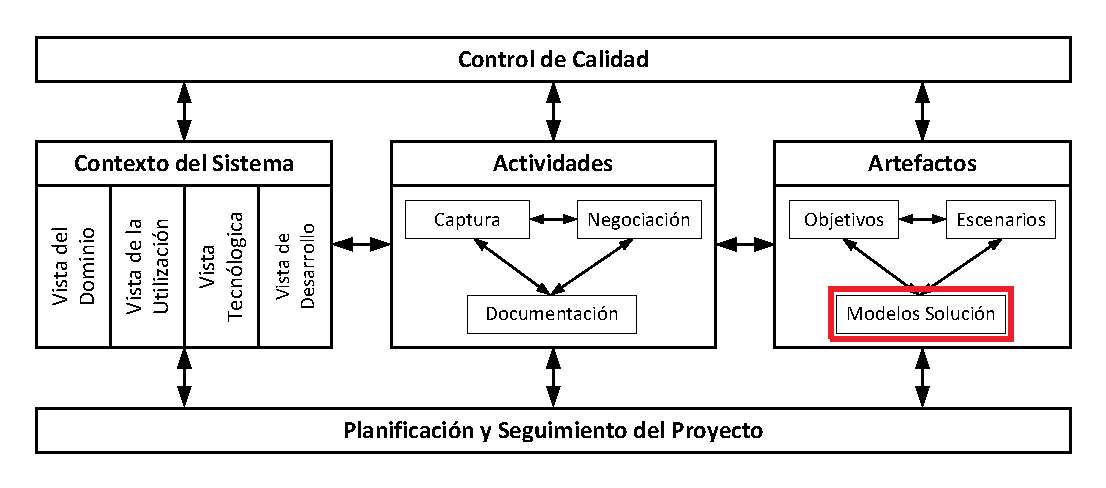
\includegraphics[width=11.5cm,keepaspectratio=true]{images/solucion.eps}}
\end{frame}

\begin{frame}[c]
    \frametitle{Modelos Orientados a la Solución}
    \begin{block}{Requisitos Orientados a la Solución}
        Los \emph{requisitos orientados a la solución} deben especificar, con un nivel suficiente de detalle, las propiedades y características del sistema a desarrollar.
    \end{block}
\end{frame}

\begin{frame}[c]
    \frametitle{Perspectivas de los Requisitos Orientados a la Solución}
    \begin{description}[<+->]
        \item[Datos] Especifica los datos que manipulará el sistema, así como las relaciones y restricciones entre ellos (EER, Clases UML).
        \item[Funcional] Especifica las funcionalidades que implementará el sistema, las relaciones entre las entradas y salidas de cada función, así como las posibles dependencias entre funciones y restricciones (flujos de datos, actividades UML).
        \item[Comportamiento] Especifica cómo reacciona un sistema a estímulos externos (máquinas de estado).
    \end{description}
\end{frame}

\begin{frame}[c]
    \frametitle{Características de los Requisitos Orientados a la Solución}
    \begin{enumerate}[<+->]
        \item Consensuados y libres de conflictos.
        \item Completos, suficientemente detallados y no ambiguos.
        \item Enfocados a crear una solución sw (generación de código).
    \end{enumerate}
\end{frame}

\section{Jerarquías de Requisitos Funcionales}

\begin{frame}
    \frametitle{Jerarquías de Requisitos}
    \only<1>{
	   \rput[lt](0,0){
	   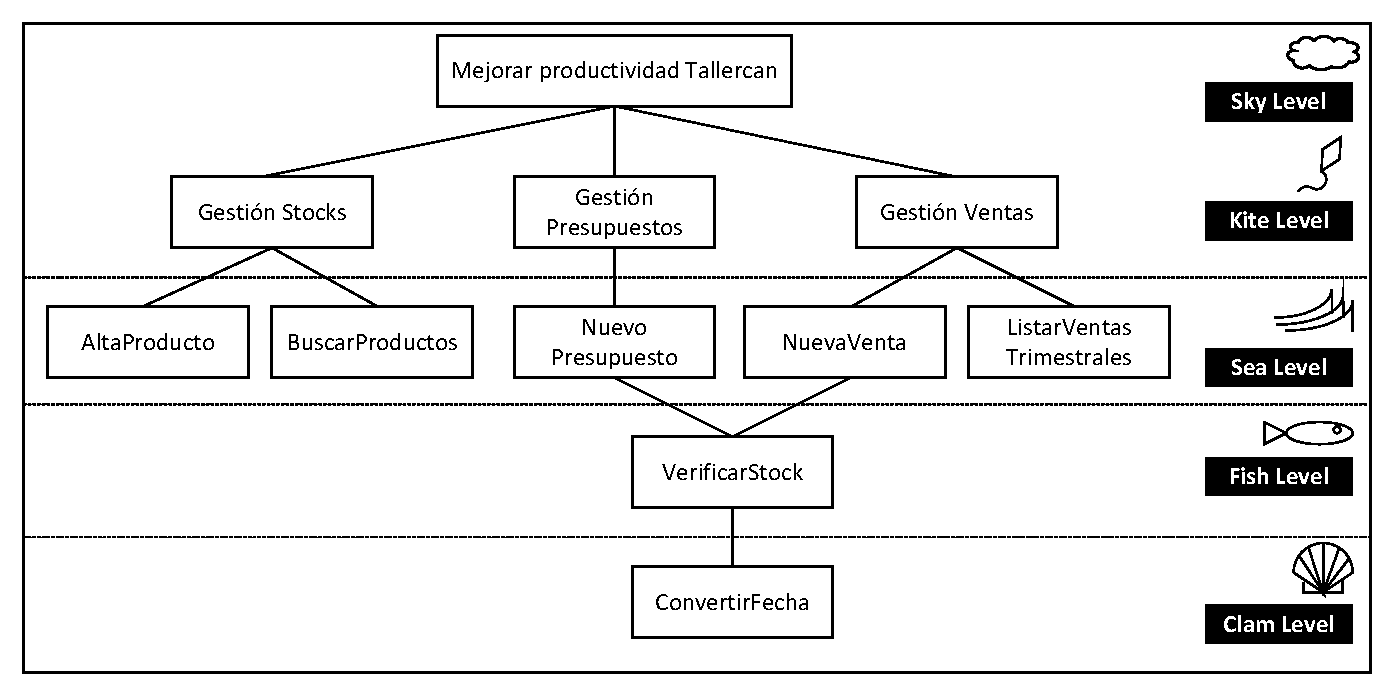
\includegraphics[width=\linewidth,keepaspectratio=true]{images/jerarquia/jerarquia00.eps}}
    }
\end{frame}

\begin{frame}
    \frametitle{Jerarquías de Requisitos}
    \only<1>{
	   \rput[lt](0,0){
	   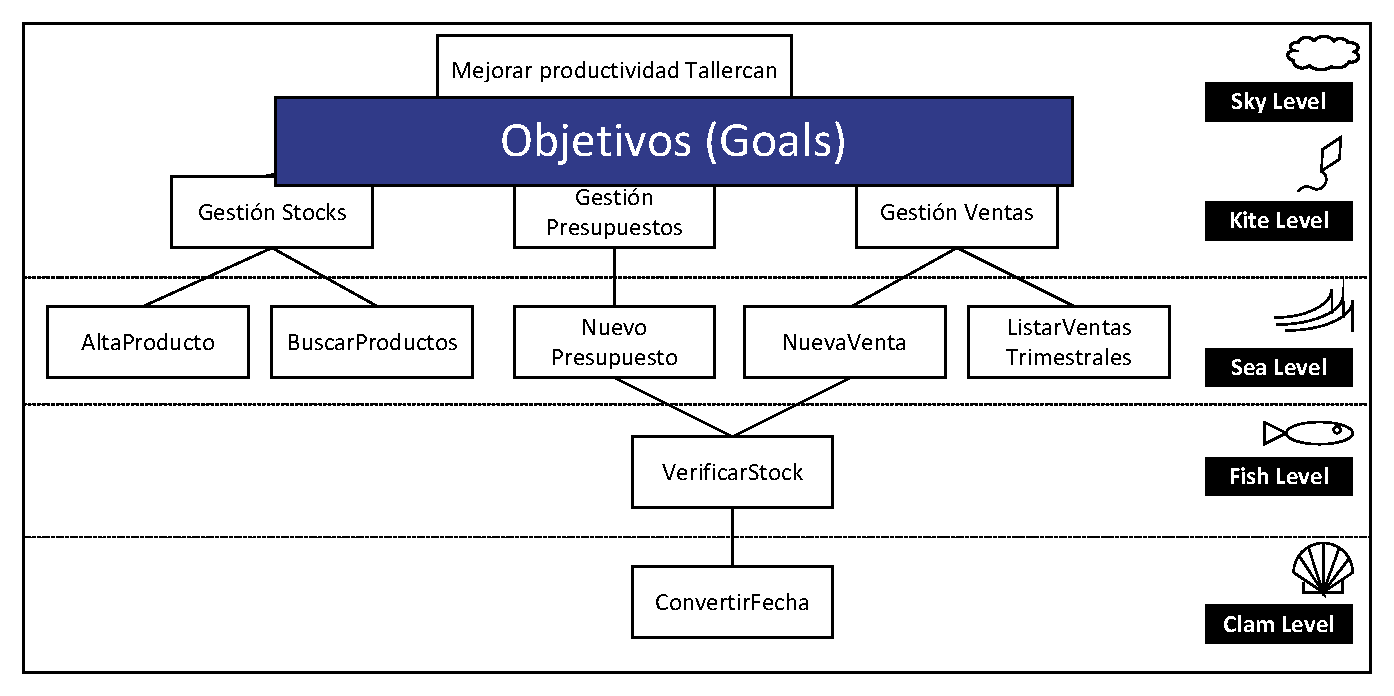
\includegraphics[width=\linewidth,keepaspectratio=true]{images/jerarquia/jerarquia01.eps}}
    }
    \only<2>{
	   \rput[lt](0,0){
	   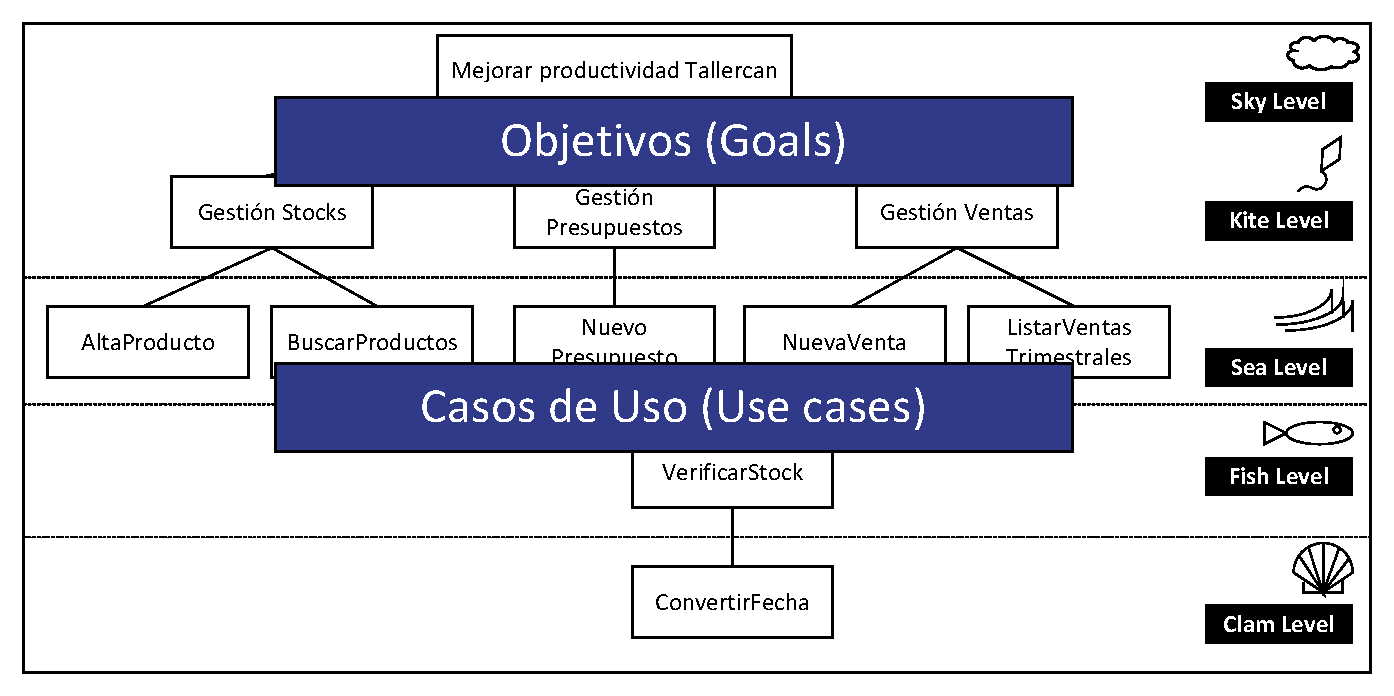
\includegraphics[width=\linewidth,keepaspectratio=true]{images/jerarquia/jerarquia02.eps}}
    }
\end{frame}

\section{Modelado y Especificación de Objetivos}

%\begin{frame}[c]
%    \frametitle{Índice - Modelado y Especificación de Objetivos}
%    \begin{enumerate}
%         \item \alert<2->{Motivación}.
%         \item Sintaxis GRL/KAOS (I): Elementos.
%         \item Sintaxis GRL/KAOS (II): Relaciones.
%         \item Elaboración de modelos orientados a objetivos.
%         \item Patrones orientados a objetivos.
%         \item Reglas de documentación de objetivos.
%    \end{enumerate}
%\end{frame}

\subsection{Introducción}

\begin{frame}
    \frametitle{Proceso de Ingeniería de Requisitos}
	\rput[lt](0,-0.5){
	   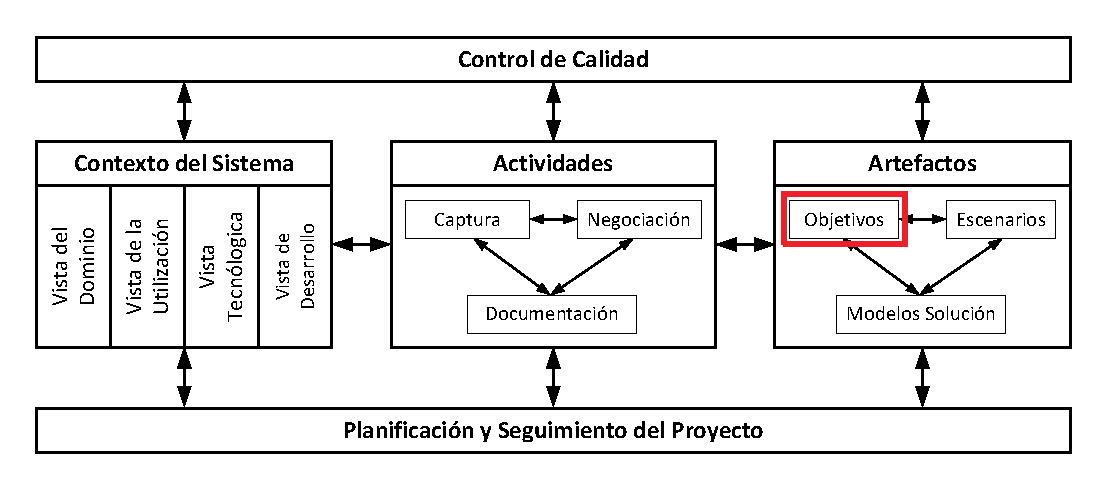
\includegraphics[width=11.5cm,keepaspectratio=true]{images/objetivos.eps}}
\end{frame}

\begin{frame}[c]
    \frametitle{Definición de Objetivo}
    \begin{block}{Objetivos~\cite{lamsweerde:2009}}
        Un \alert{\emph{objetivo}} de un sistema software es una descripción prescriptiva de un propósito que dicho sistema debe satisfacer mediante la cooperación de sus elementos constituyentes.
    \end{block}
%    \uncover<2->{
%    \begin{block}{Tipos de Objetivos~\cite{lamsweerde:2009}}
%        \begin{description}
%           \item<3->[Achieve] Especifican comportamientos donde se debe alcanzar, más tarde o más temprano, una cierta
%                              condición siempre y cuando se dé otra condición previa.
%            \item<4->[Maintain] Especifican comportamientos que se deben encargar de mantener una cierta condición
%                              mientras se dé otra  condición.
%            \item<5->[Avoid] Especifican comportamientos que deben evitar una cierta condición mientras se dé otra condición.
%        \end{description}
%    \end{block}
%    }
\end{frame}

\subsection[Sintaxis GRL/KAOS (I)]{Sintaxis GRL/KAOS - Elementos Básicos}

\begin{frame}
    \frametitle{Modelado de Objetivos con GRL/KAOS}
    \begin{block}{Goal Requirements Language (GRL)}
        \emph{Goal Requirements Language} es un lenguaje de modelado de objetivos, basado en \emph{i*}, integrado dentro del lenguaje \emph{URN (User Requirements Notation)}, que es actualmente estándar ITU (\emph{International Telecommunication Union}).
    \end{block}
    \uncover<2->{
    \begin{block}{Knowledge Acquisition in autOmated Specification of software (KAOS)}
        \emph{KAOS} es una metodología con un lenguaje propio de modelado de objetivos, producida por el grupo de investigación del Prof. van Lamswerdee.
    \end{block}
    }
\end{frame}

\begin{frame}[c]
    \frametitle{Sintaxis GRL/KAOS - Objetivo}
    \begin{block}{Objetivo (duro)}
        Un \alert{\emph{objetivo (duro)}} de un sistema sw es un objetivo cuya satisfacción debe alcanzarse de manera absoluta; y que, además,
        no puede satisfacerse parcialmente en la mayoría de los casos.
        \ \\
        \ \\
        \begin{columns}[c]
            \begin{column}{0.50\linewidth}
                \centering 
\includegraphics[width=0.5\columnwidth,keepaspectratio=true]{images/objetivos/goal(GRL).eps}
            \end{column}
            \begin{column}{0.50\linewidth}
                \centering 
\includegraphics[width=0.5\columnwidth,keepaspectratio=true]{images/objetivos/goal(KAOS).eps}
            \end{column}
        \end{columns}
    \end{block}
\end{frame}

\begin{frame}[c]
    \frametitle{Sintaxis GRL/KAOS - Objetivo Blando}
    \begin{block}{Objetivo Blando}
        Un \alert{\emph{objetivo blando}} de un sistema sw es un objetivo cuya satisfacción no puede alcanzar de forma absoluta, de forma que es satisfecho hasta un cierto grado, el cual suele venir determinado por un \emph{criterio de satisfacción}.
        \ \\
        \ \\
        \begin{columns}[c]
            \begin{column}{0.50\linewidth}
                \centering 
\includegraphics[width=0.5\columnwidth,keepaspectratio=true]{images/objetivos/softgoal(GRL).eps}
            \end{column}
            \begin{column}{0.50\linewidth}
                \centering 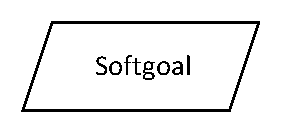
\includegraphics[width=0.5\columnwidth,keepaspectratio=true]{images/objetivos/softgoal(KAOS).eps}
            \end{column}
        \end{columns}
    \end{block}
\end{frame}

\begin{frame}[c]
	\frametitle{Sintaxis GRL/KAOS - Tarea}
	\begin{block}{Tarea/Operación}
		Un \alert{\emph{tarea}} u \alert{\emph{operación}} representa una forma concreta de llevar a cabo una acción que afecta al estado del sistema.
		Las tareas representan la materialización de un objetivo.
		\ \\
		\ \\
		\begin{columns}[c]
			\begin{column}{0.50\linewidth}
				\centering 
\includegraphics[width=0.5\columnwidth,keepaspectratio=true]{images/objetivos/task(GRL).eps}
			\end{column}
			\begin{column}{0.50\linewidth}
				\centering 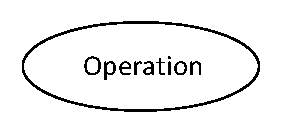
\includegraphics[width=0.5\columnwidth,keepaspectratio=true]{images/objetivos/operation(KAOS).eps}
			\end{column}
		\end{columns}
	\end{block}
\end{frame}

\begin{frame}[c]
    \frametitle{Sintaxis GRL/KAOS - Relaciones AND}
    \begin{block}{Refinamiento AND}
        Un \alert{\emph{refinamiento AND}} descompone un objetivo padre en diversos subobjetivos hijos, los cuales han de satisfacerse todos para que el padre pueda ser satisfecho. Si la satisfacción de los objetivos es suficiente para la satisfacción del objetivo padre, se dice que el refinamiento es \emph{completo}.
        \ \\
        \ \\
        \begin{columns}[c]
            \begin{column}{.50\linewidth}
                \centering 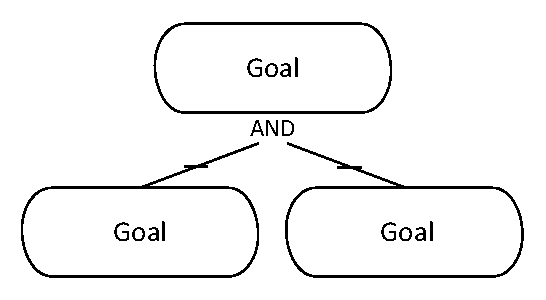
\includegraphics[width=0.65\columnwidth,keepaspectratio=true]{images/objetivos/andRef(GRL).eps}
            \end{column}
            \begin{column}{.50\linewidth}
                \centering 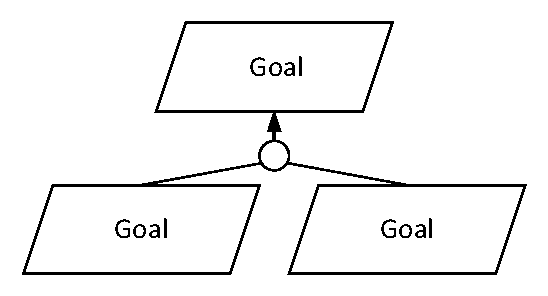
\includegraphics[width=0.65\columnwidth,keepaspectratio=true]{images/objetivos/andRef(KAOS).eps}
            \end{column}
        \end{columns}
        \begin{columns}[c]
            \begin{column}{.50\linewidth}
            \end{column}
            \begin{column}{.50\linewidth}
                \centering 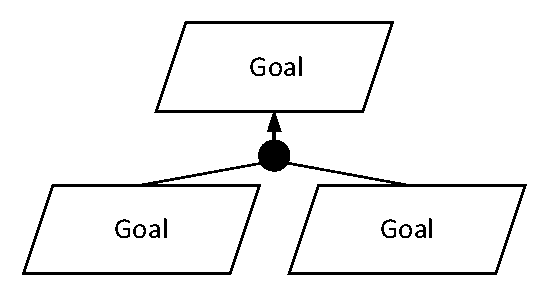
\includegraphics[width=0.65\columnwidth,keepaspectratio=true]{images/objetivos/andRef(complete)(KAOS).eps}
            \end{column}
        \end{columns}
     \end{block}
\end{frame}

\begin{frame}[c]
    \frametitle{Sintaxis GRL/KAOS - Relaciones OR}
    \begin{block}{Refinamiento OR}
        Un \alert{\emph{refinamiento OR}} descompone un objetivo padre en diversos subobjetivos hijos, de los cuales, al menos uno debe satisfacerse para que el padre pueda ser satisfecho. Las relaciones OR representan diferentes maneras de alcanzar un mismo objetivo.
        \ \\
        \ \\
        \begin{columns}[c]
            \begin{column}{0.50\linewidth}
                \centering 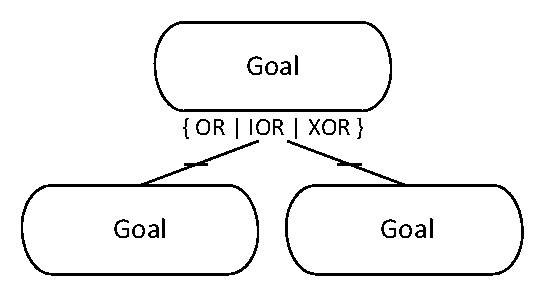
\includegraphics[width=0.65\columnwidth,keepaspectratio=true]{images/objetivos/orRef(GRL).eps}
            \end{column}
            \begin{column}{0.50\linewidth}
                \centering 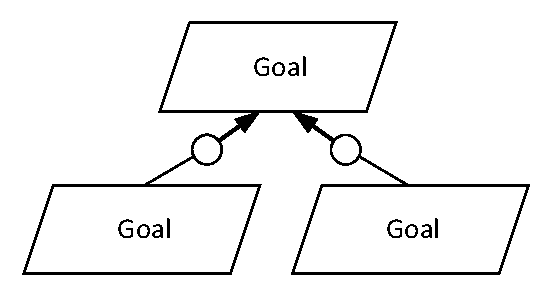
\includegraphics[width=0.65\columnwidth,keepaspectratio=true]{images/objetivos/orRef(KAOS).eps}
            \end{column}
        \end{columns}
        \begin{columns}[c]
            \begin{column}{0.50\linewidth}
                \centering 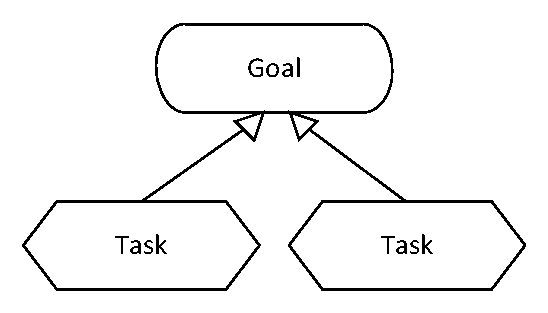
\includegraphics[width=0.65\columnwidth,keepaspectratio=true]{images/objetivos/meansEnd(GRL).eps}
            \end{column}
            \begin{column}{0.50\linewidth}
            \end{column}
        \end{columns}
     \end{block}
\end{frame}

\begin{frame}[c]
    \frametitle{Sintaxis GRL/KAOS - Contribución}
    \begin{block}{Contribución (GRL)}
        Una \alert{\emph{contribución}} describe el impacto intencionado que un elemento posee sobre un determinado objetivo.
        \ \\
        \ \\
        \begin{columns}[c]
            \begin{column}{0.5\linewidth}
                \centering 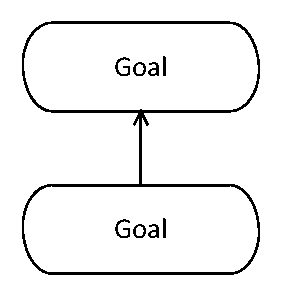
\includegraphics[width=0.35\columnwidth,keepaspectratio=true]{images/objetivos/contribution(GRL).eps}
            \end{column}
            \begin{column}{0.5\linewidth}
            \end{column}
        \end{columns}
    \end{block}
\end{frame}

\begin{frame}[c]
    \frametitle{Sintaxis GRL/KAOS - Correlación}
    \begin{block}{Correlación}
        Una \alert{\emph{correlación}} describe el impacto no intencionado que un determinado elemento tiene sobre un determinado objetivo.
        \ \\
        \ \\
        \begin{columns}[c]
            \begin{column}{0.5\linewidth}
                \centering 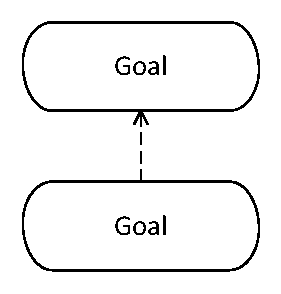
\includegraphics[width=0.35\columnwidth,keepaspectratio=true]{images/objetivos/correlation(GRL).eps}
            \end{column}
            \begin{column}{0.5\linewidth}
                \centering 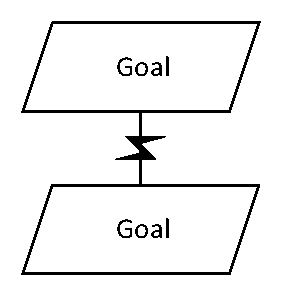
\includegraphics[width=0.35\columnwidth,keepaspectratio=true]{images/objetivos/contribution(KAOS).eps}
            \end{column}
        \end{columns}
        \begin{columns}[c]
            \begin{column}{0.50\linewidth}
            \end{column}
            \begin{column}{0.50\linewidth}
                \centering 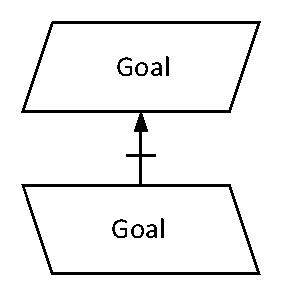
\includegraphics[width=0.35\columnwidth,keepaspectratio=true]{images/objetivos/contribution(2)(KAOS).eps}
            \end{column}
        \end{columns}
    \end{block}
\end{frame}

\begin{frame}[c]
    \frametitle{Sintaxis GRL/KAOS - Escala de Contribución}
    \begin{block}{Tipos de Contribución/Correlación (GRL)}
        \begin{description}
            \item[Make] La contribución es positiva y suficiente.
            \item[Some Positive] La contribución es positiva, pero no suficiente.
            \item[Help] La contribución es positiva, pero no significativa.
            \item[Unknown] Un elemento afecta al otro, pero no se sabe cómo.
            \item[Hurt] La contribución es negativa, pero no significativa.
            \item[Some Negative] La contribución es negativa, pero no impide la satisfacción del elemento destino.
            \item[Break] La contribución es negativa e impide la satisfacción del elemento destino.
        \end{description}
        \begin{columns}[c]
            \begin{column}{\linewidth}
                \centering 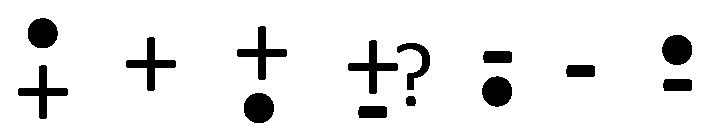
\includegraphics[width=0.70\columnwidth,keepaspectratio=true]{images/objetivos/influence(GRL).eps}
            \end{column}
        \end{columns}
    \end{block}
\end{frame}

\subsection{Análisis de Influencias entre Objetivos}

\begin{frame}[t]
	\frametitle{Influencias entre Objetivos}
	\only<1>{
		\rput[lt](0,0){
			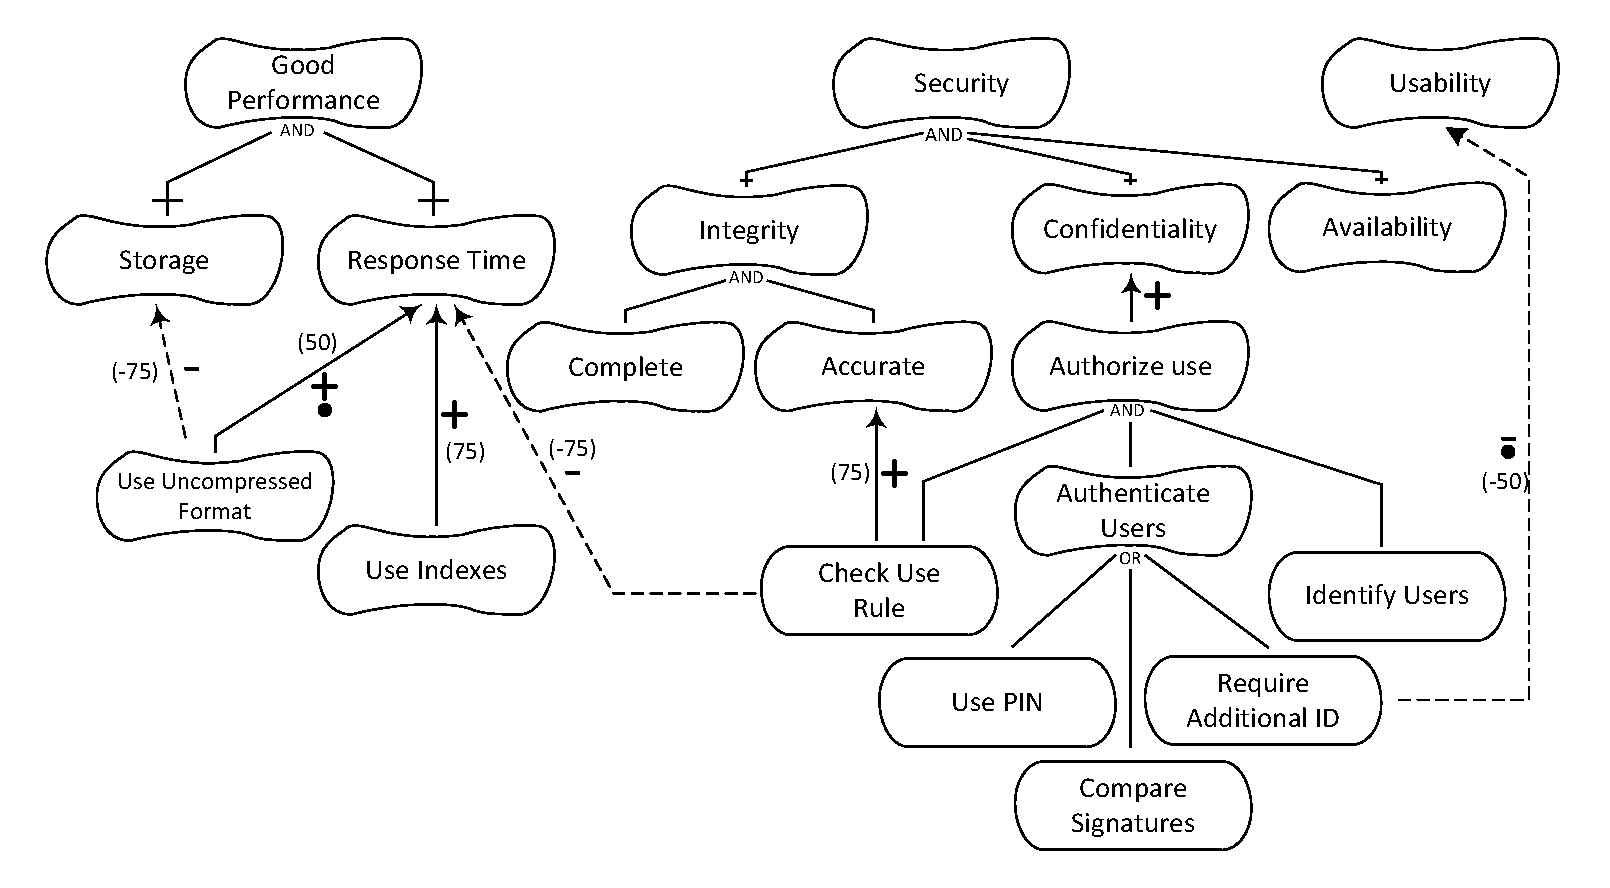
\includegraphics[width=12cm,keepaspectratio=true]{images/influences/nfrInfluences.eps}}
	}
\end{frame}

\begin{frame}[c]
	\frametitle{Algoritmo de Hao}
	\begin{block}{Regla de Evaluación de Objetivos/Tareas Hoja}
		\begin{center}
			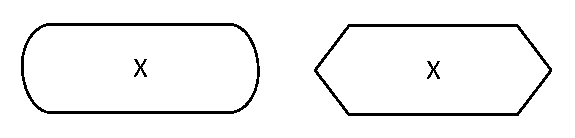
\includegraphics[width=0.5\linewidth,keepaspectratio=true]{images/influences/leafGoal.eps}
		\end{center}
		\begin{equation*}
		V(X) =
		\begin{cases}
		100, \text{si\ } X \text{\ está seleccionado} \\
		0, \text{otro caso}
		\end{cases}
		\end{equation*}
		\ \\ \ \\
	\end{block}
\end{frame}

\begin{frame}[c]
	\frametitle{Evaluación de Relaciones AND}
	\begin{block}{Regla de Evaluación de Relación AND}
		\begin{center}
			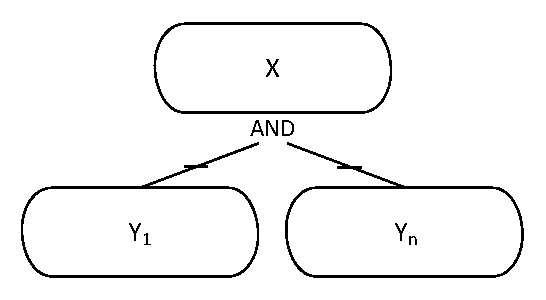
\includegraphics[width=0.4\linewidth,keepaspectratio=true]{images/influences/andRelationship.eps}
		\end{center}
		\begin{equation*}
		V(X) = min_{i=1}^{n} V(Y_{i})
		\end{equation*}
		\ \\ \ \\
	\end{block}
\end{frame}

\begin{frame}[c]
	\frametitle{Evaluación de Relaciones OR}
	\begin{block}{Regla de Evaluación de Relación OR (Hao)}
		\begin{center}
			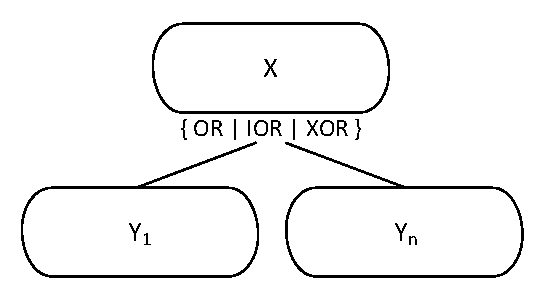
\includegraphics[width=0.4\linewidth,keepaspectratio=true]{images/influences/orRelationship.eps}
		\end{center}
		\begin{equation*}
		V(X) = max_{i=1}^{n} V(Y_{i})
		\end{equation*}
		\ \\ \ \\
	\end{block}
\end{frame}

\begin{frame}[c]
	\frametitle{Evaluación de Contribuciones/Correlaciones}
	\begin{block}{Regla de Evaluación de Contribuciones}
		\begin{center}
			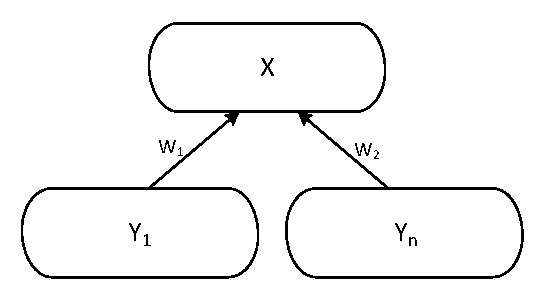
\includegraphics[width=0.4\linewidth,keepaspectratio=true]{images/influences/contributionRelationship.eps}
		\end{center}
		\begin{equation*}
		V(X) = max(-100,min(100,\frac{\sum_{i=1}^{n} V(Y_{i})*W_{i}}{100}))
		\end{equation*}
		\ \\ \ \\
	\end{block}
\end{frame}

\begin{frame}
	\frametitle{Ejemplo: Índices y Verificación de Firmas}
	\only<1>{
		\rput[lt](0,0){
			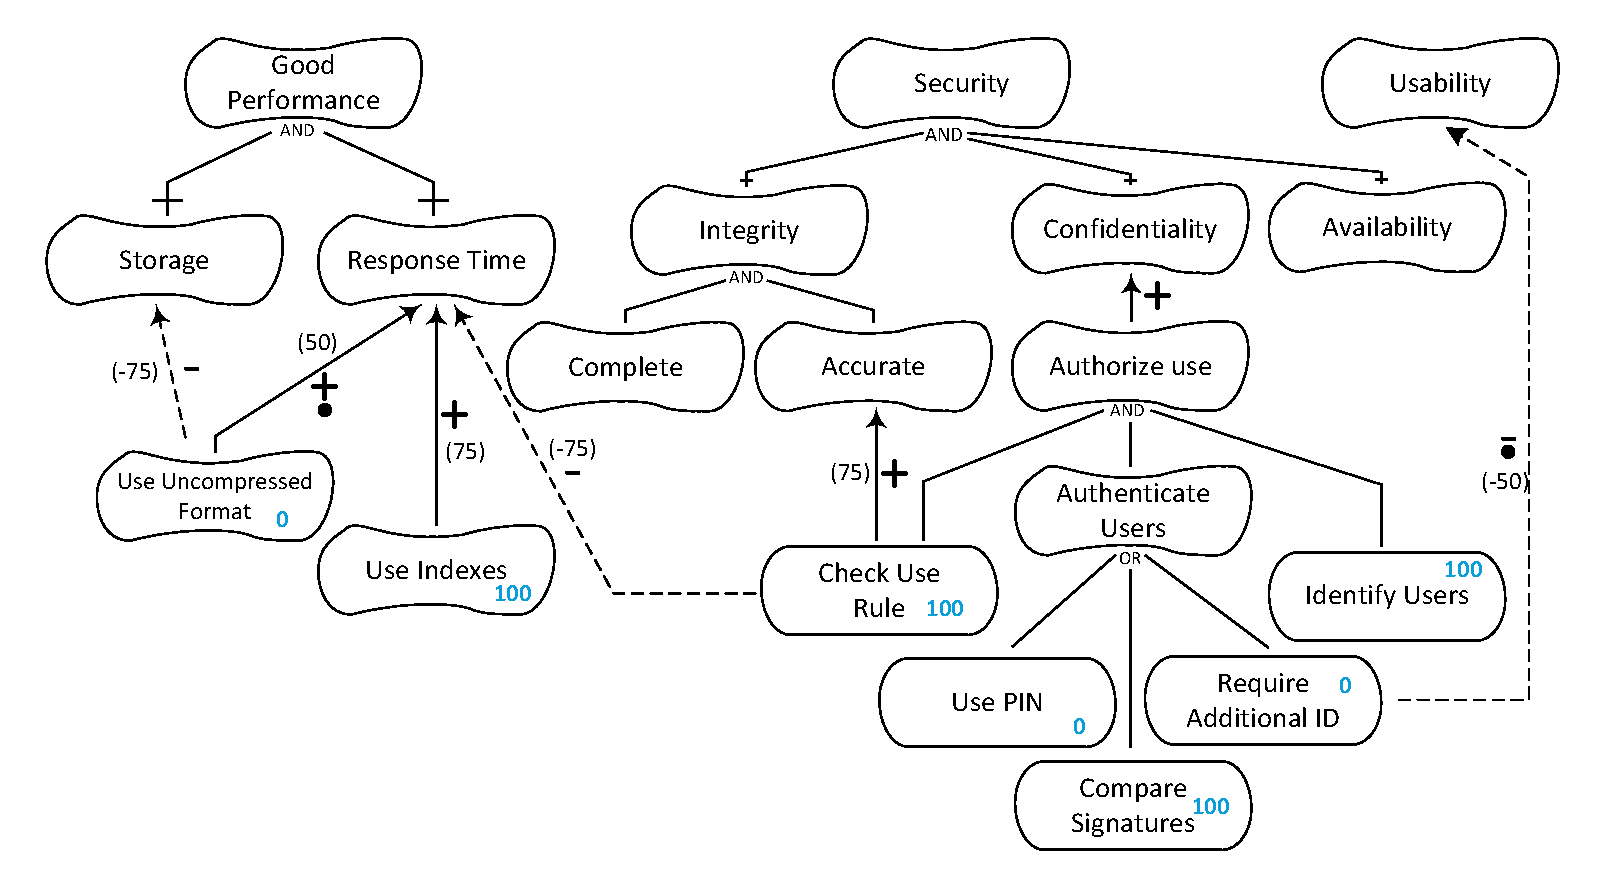
\includegraphics[width=11.5cm,keepaspectratio=true]{images/influences/example01_00.eps}}
	}
	\only<2>{
		\rput[lt](0,0){
			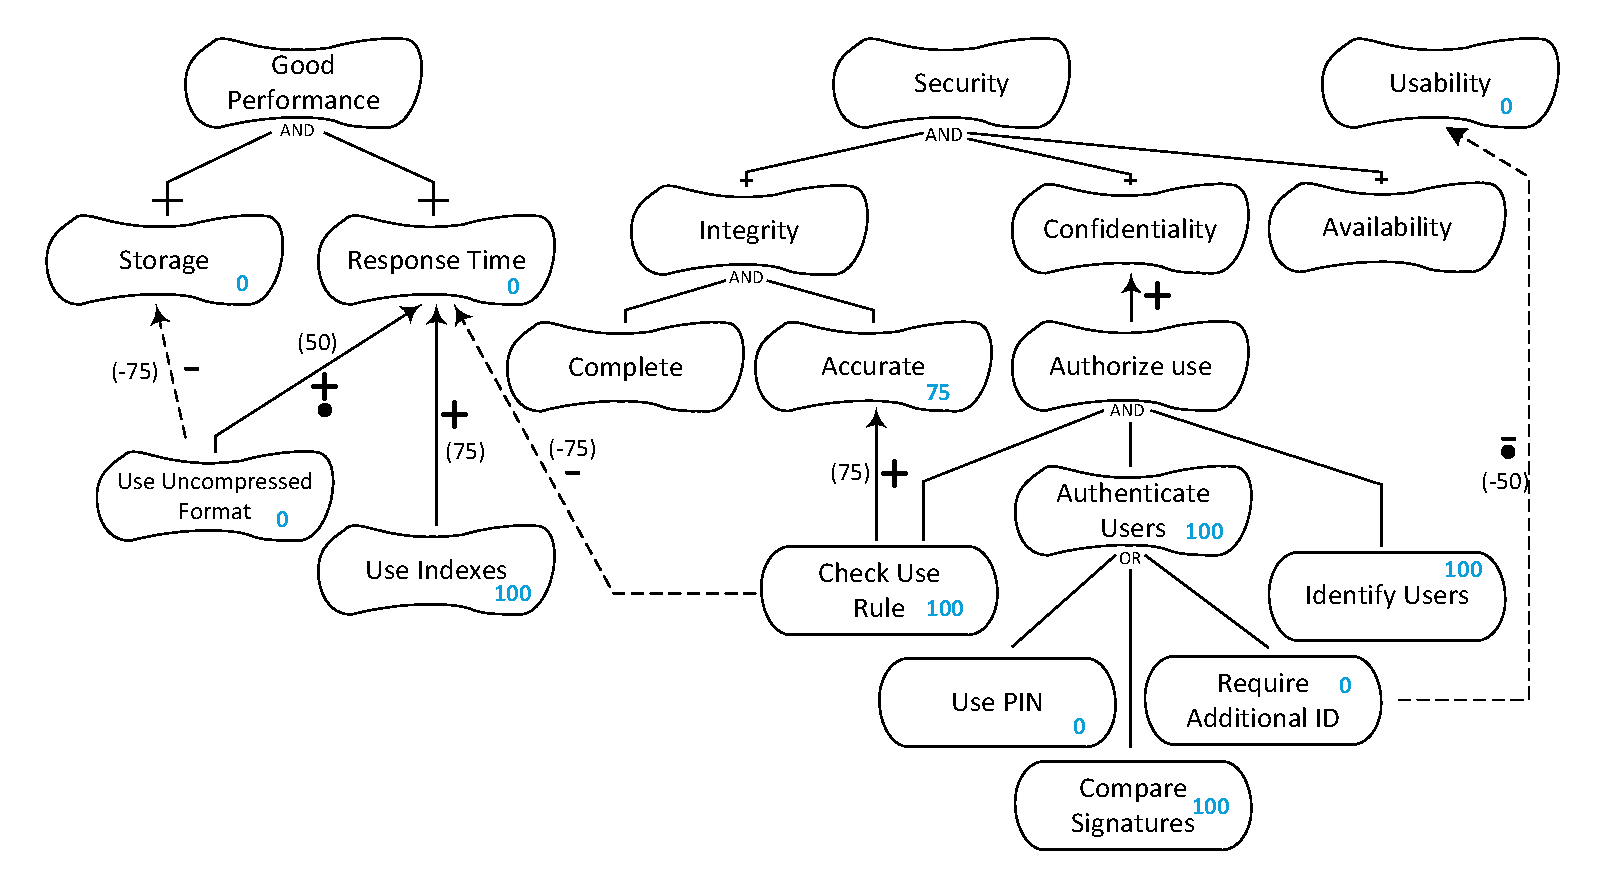
\includegraphics[width=11.5cm,keepaspectratio=true]{images/influences/example01_01.eps}}
	}
	\only<3>{
		\rput[lt](0,0){
			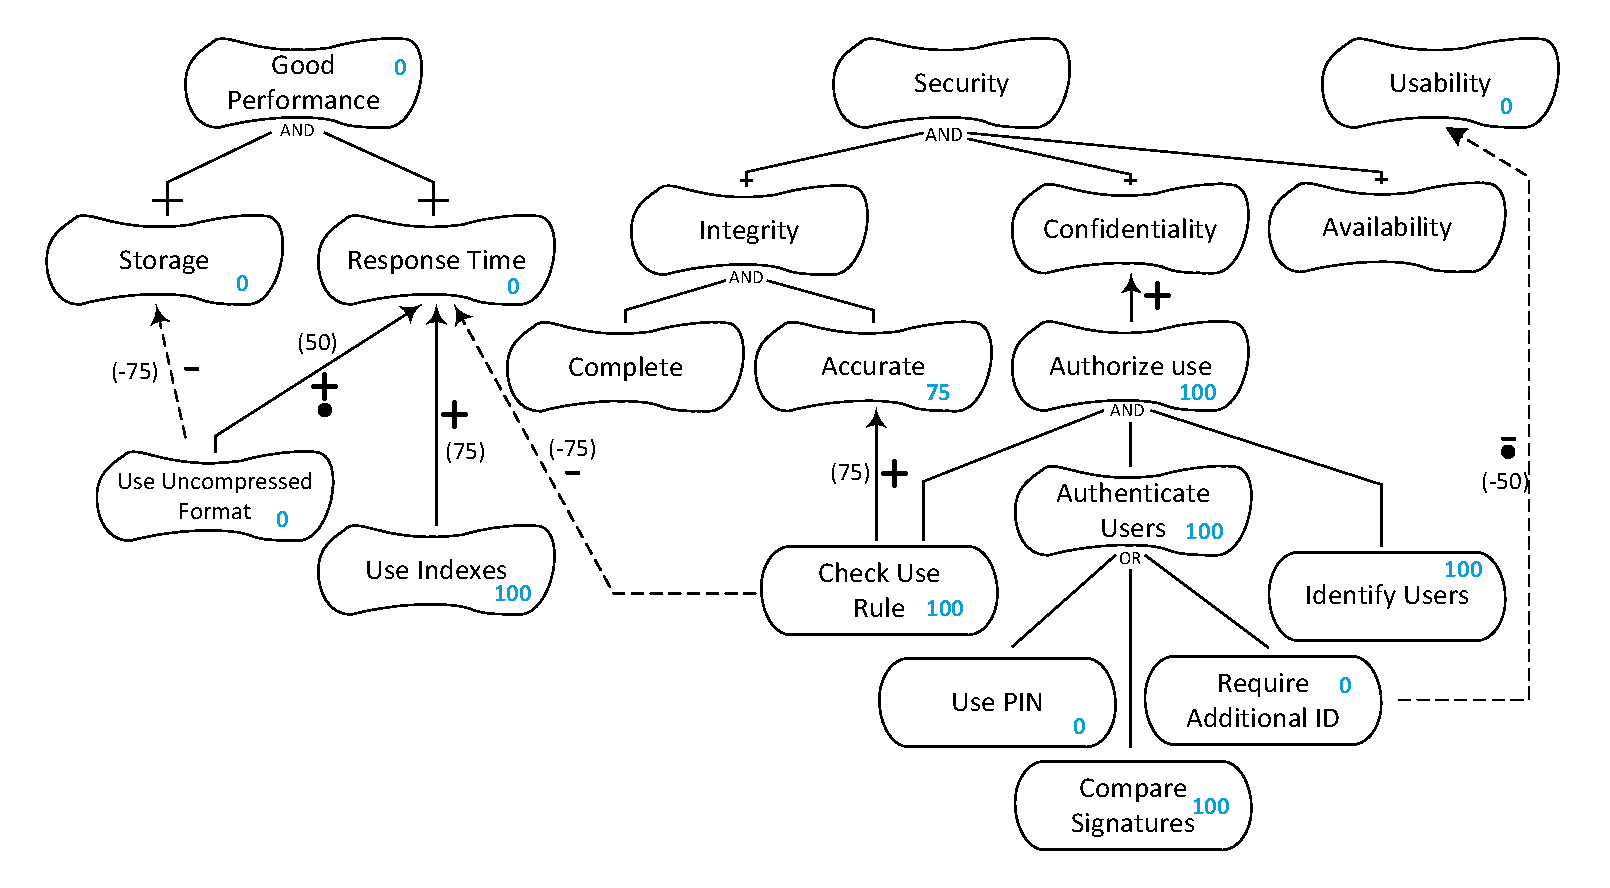
\includegraphics[width=11.5cm,keepaspectratio=true]{images/influences/example01_02.eps}}
	}
	\only<4>{
		\rput[lt](0,0){
			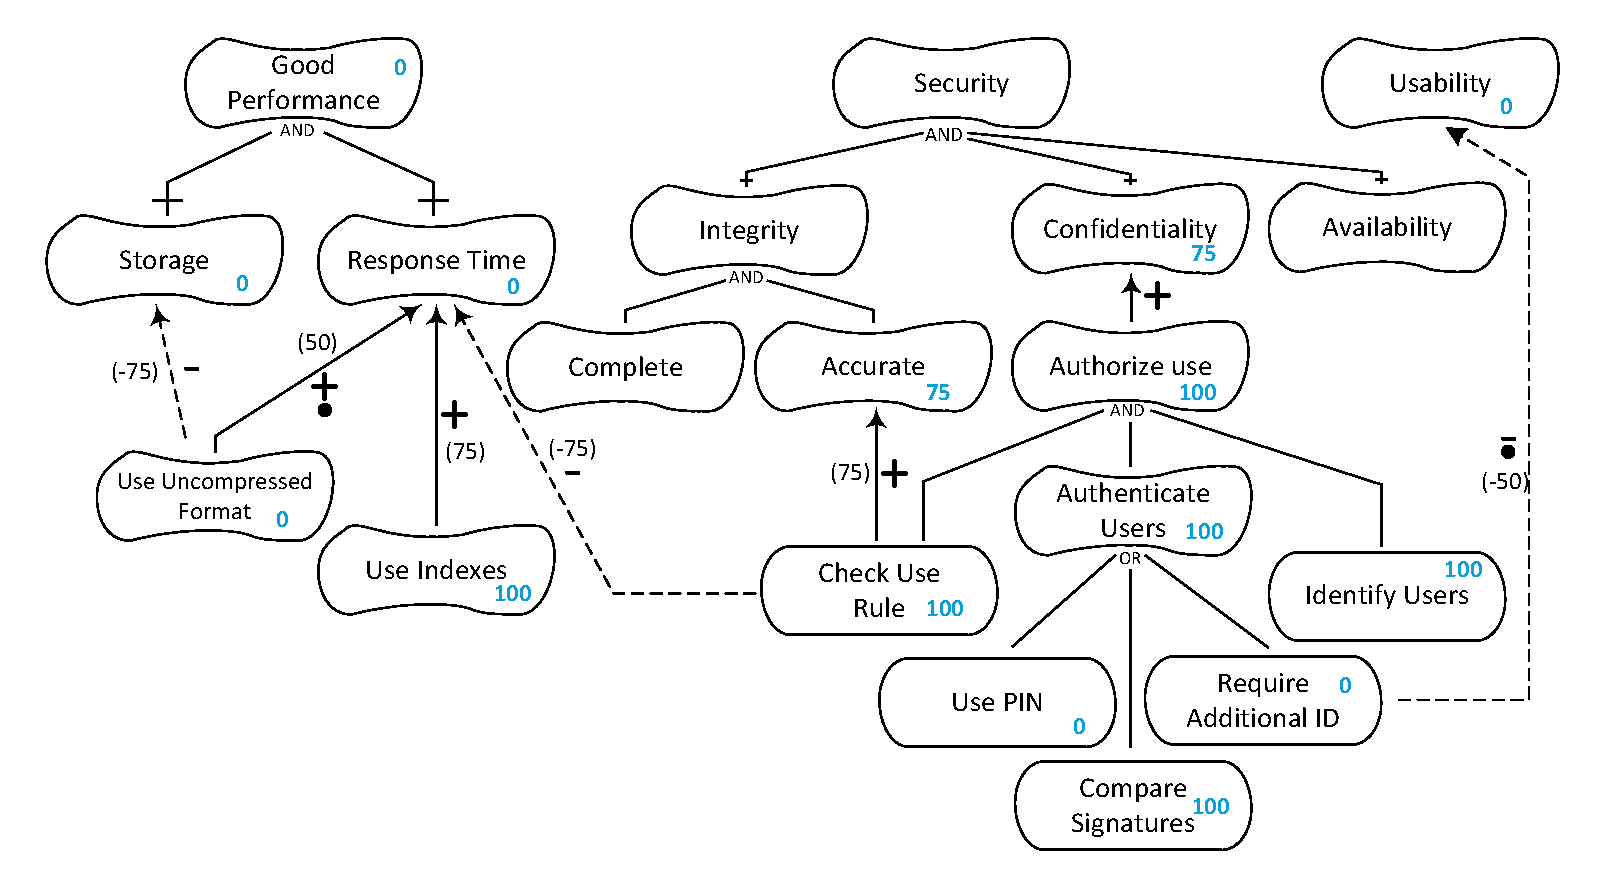
\includegraphics[width=11.5cm,keepaspectratio=true]{images/influences/example01_03.eps}}
	}
\end{frame}

\subsection[Sintaxis GRL/KAOS (II)]{Sintaxis GRL/KAOS - Elementos Avanzados}

\begin{frame}[c]
    \frametitle{Sintaxis GRL/KAOS - Recurso}
    \begin{block}{Recurso/Entidad}
        Un \alert{\emph{recurso}} o \alert{\emph{entidad}} es un elemento físico o lógico que forma parte del sistema sw a construir o de su contexto.
        \ \\
        \ \\
        \begin{columns}[c]
            \begin{column}{0.50\linewidth}
                \centering 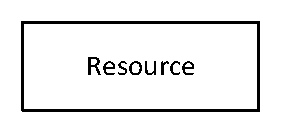
\includegraphics[width=0.5\columnwidth,keepaspectratio=true]{images/objetivos/resource(GRL).eps}
            \end{column}
            \begin{column}{0.50\linewidth}
                \centering 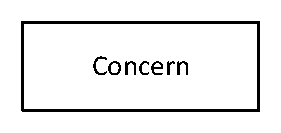
\includegraphics[width=0.5\columnwidth,keepaspectratio=true]{images/objetivos/concern(KAOS).eps}
            \end{column}
        \end{columns}
    \end{block}
\end{frame}

\begin{frame}[c]
    \frametitle{Sintaxis GRL/KAOS - Hipótesis}
    \begin{block}{Creencia/Hipótesis o Propiedad}
        Una \alert{\emph{creencia}}, \alert{\emph{hipótesis}} o \alert{\emph{propiedad}} es una predicado sobre el dominio del sistema. Se utiliza normalmente para justificar una decisión. Las \emph{propiedades} se diferencian de las \emph{hipótesis} o \emph{creencias} en que las primeras están probadas.
        \ \\
        \ \\
        \begin{columns}[c]
            \begin{column}{0.50\linewidth}
                \centering 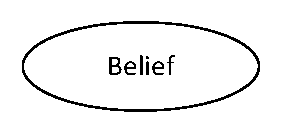
\includegraphics[width=0.5\columnwidth,keepaspectratio=true]{images/objetivos/belief(GRL).eps}
            \end{column}
            \begin{column}{0.50\linewidth}
                \centering 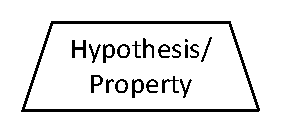
\includegraphics[width=0.5\columnwidth,keepaspectratio=true]{images/objetivos/hypothesis(KAOS).eps}
            \end{column}
        \end{columns}
    \end{block}
\end{frame}

\begin{frame}[c]
    \frametitle{Sintaxis GRL/KAOS - Agente}
    \begin{block}{Actor/Agente}
        Un \alert{\emph{actor}} o \alert{\emph{agente}} es una entidad (persona o sistema) que tiene intereses o expectativas sobre el sistema y/o ejecuta acciones para satisfacer unos determinados objetivos.
        \ \\
        \ \\
        \begin{columns}[c]
            \begin{column}{0.50\linewidth}
                \centering 
\includegraphics[width=0.50\columnwidth,keepaspectratio=true]{images/objetivos/actor(GRL).eps}
            \end{column}
            \begin{column}{0.50\linewidth}
                \centering 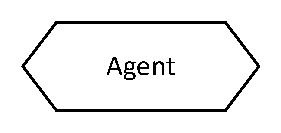
\includegraphics[width=0.50\columnwidth,keepaspectratio=true]{images/objetivos/agent(KAOS).eps}
            \end{column}
        \end{columns}
        \begin{columns}[c]
            \begin{column}{0.50\linewidth}
            \end{column}
            \begin{column}{0.50\linewidth}
                \centering 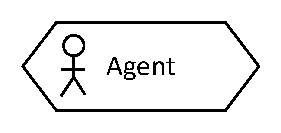
\includegraphics[width=0.50\columnwidth,keepaspectratio=true]{images/objetivos/enviromentalAgent(KAOS).eps}
            \end{column}
        \end{columns}
     \end{block}
\end{frame}

\begin{frame}[c]
    \frametitle{Sintaxis GRL/KAOS - Requisito}
    \begin{block}{Requisito o Expectativa (KAOS)}
        Un \alert{\emph{requisito}} es un objetivo que es responsabilidad de un único agente del sistema a construir. Una \alert{\emph{expectativa}} es un objetivo que es responsabilidad de un único agente del entorno del sistema a construir.
        \ \\
        \ \\
        \begin{columns}[c]
            \begin{column}{0.50\linewidth}
            \end{column}
            \begin{column}{0.50\linewidth}
                \centering 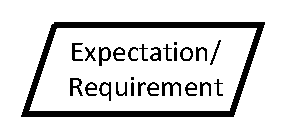
\includegraphics[width=0.50\columnwidth,keepaspectratio=true]{images/objetivos/expectation(KAOS).eps}
            \end{column}
        \end{columns}
     \end{block}
\end{frame}

\begin{frame}[c]
    \frametitle{Sintaxis GRL/KAOS - Obstáculo}
    \begin{block}{Obstáculo (KAOS)}
        Un \alert{\emph{obstáculo}}  a un objetivo es una situación factible dentro de un sistema software, que en caso de que ocurra, impide la satisfacción de dicho objetivo.
        \ \\
        \ \\
        \begin{columns}[c]
            \begin{column}{0.50\linewidth}
            \end{column}
            \begin{column}{0.50\linewidth}
                \centering 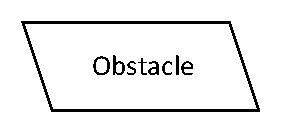
\includegraphics[width=0.50\columnwidth,keepaspectratio=true]{images/objetivos/obstacle(KAOS).eps}
            \end{column}
        \end{columns}
     \end{block}
\end{frame}

\begin{frame}[c]
    \frametitle{Sintaxis GRL/KAOS - Responsabilidades}
    \begin{block}{Asignación Responsabilidad (KAOS)}
        Una \alert{\emph{asignación de responsabilidad}} entre un objetivo y un agente indica que el agente es el responsable último de la satisfacción de dicho objetivo.
        \ \\
        \ \\
        \begin{columns}[c]
            \begin{column}{0.50\linewidth}
            \end{column}
            \begin{column}{0.50\linewidth}
                \centering 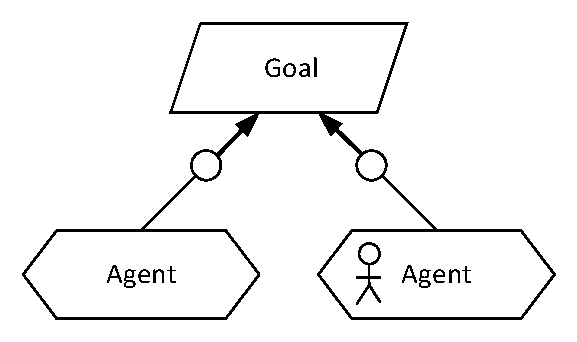
\includegraphics[width=0.65\columnwidth,keepaspectratio=true]{images/objetivos/responsabilityAsig(KAOS).eps}
            \end{column}
        \end{columns}
    \end{block}
\end{frame}

\begin{frame}[t]
    \frametitle{Sintaxis GRL/KAOS - Dependencias GRL}
    \begin{block}{Dependencia}
        Una \alert{\emph{dependencia}} describe como un elemento de un actor depende de otro  elemento de otro actor.
        \ \\
        \ \\
        \begin{columns}
            \begin{column}{\linewidth}
                \centering 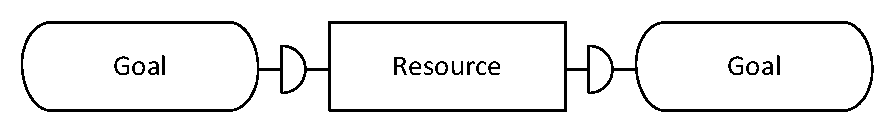
\includegraphics[width=0.75\columnwidth,keepaspectratio=true]{images/objetivos/dependency(GRL).eps}
            \end{column}
        \end{columns}
    \end{block}
\end{frame}

%%\begin{frame}
%%    \frametitle{Diagrama GRL}
%%    \begin{center}
%%        \includegraphics[width=0.80\linewidth,keepaspectratio=true]{images/grl/example.eps}
%%    \end{center}
%%\end{frame}

\subsection[Proceso de Modelado de Objetivos]{Proceso de Elaboración de Modelos Orientados a Objetivos}

\begin{frame}[c]
    \frametitle{Identificación de Objetivos}
    \begin{enumerate}[<+->]
         \item Identificar objetivos estratégicos y problemas del sistema actual.
         \item Identificar deseos y esperanzas de cada \emph{stakeholder}.
         \item Buscar palabras claves en la documentación a analizar (oral o escrita).
         \item Análisis de alternativas.
         \item Utilizar categorías predefinidas (no funcionales).
    \end{enumerate}
\end{frame}

\begin{frame}[c]
    \frametitle{Refinado de Objetivos}
    \begin{enumerate}[<+->]
         \item Preguntar \emph{cómo} para identificar subobjetivos.
         \item Preguntar \emph{por qué} para identificar superobjetivos.
         \item Dividir responsabilidades.
         \item Análisis de obstáculos, amenazas y conflictos.
         %% \item Analizar si las condiciones \emph{si} son convertibles en \emph{si y sólo si}.
         %% \item Analizar la contra guarda de las condiciones \emph{si}.
    \end{enumerate}
\end{frame}

\begin{frame}[c]
    \frametitle{Criterio de Parada}
    \begin{enumerate}[<+->]
         \item Parar cuando un objetivo esté el nivel del mar.
         \item Parar cuando un objetivo esté fuera del contexto del sistema.
    \end{enumerate}
\end{frame}

\begin{frame}[c]
    \frametitle{Fallos comunes}
    \begin{enumerate}[<+->]
         \item Confundir objetivos y operaciones.
         \item Confundir descomposiciones AND con descomposiciones OR.
         \item Abusar de relaciones AND y OR.
         \item Imprecisiones.
         %% sobreespecificaciones.
         \item Modelar secuencia temporal como dependencias.
    \end{enumerate}
\end{frame}

\begin{frame}[c]
    \frametitle{Reglas para la Documentación de Objetivos}
    \begin{enumerate}[<+->]
        \item Concisión
        \item Evitar usar oraciones pasivas (inglés) o impersonales.
        \item Documentar intenciones de forma precisa y verificable.
        \item Redactar explícitamente el valor de cada objetivo.
        \item Evitar introducir restricciones innecesarias.
    \end{enumerate}
\end{frame}

\subsection{Ventajas de los Objetivos}

\begin{frame}[c]
	\frametitle{Ventajas de los Objetivos}
	\begin{enumerate}[<+->]
		\item Facilita el refinamiento de la \emph{visión del sistema}.
		\item Dirige y organiza el proceso de captura de requisitos.
		\item Favorece la identificación y análisis de alternativas.
		\item Permite detectar requisitos irrelevantes.
		\item Permite justificar la existencia de los requisitos.
		\item Permite evaluar la completitud de una especificación de requisitos.
		\item Favorece la identificación y resolución de conflictos.
		\item Los objetivos poseen una alta estabilidad con respecto a los cambios en el sistema.
	\end{enumerate}
\end{frame}

\subsection{Patrones Orientados a Objetivos}

\begin{frame}[c]
    \frametitle{Patrón Punto Intermedio}
    \begin{center}
        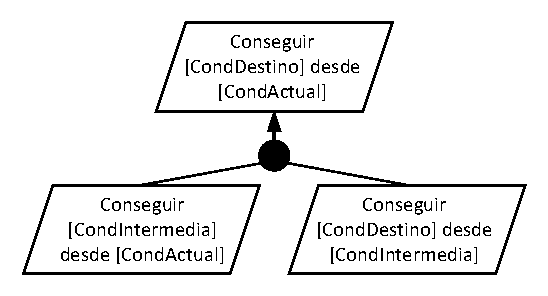
\includegraphics[width=0.70\linewidth,keepaspectratio=true]{images/objetivos/milestonePattern.eps}
    \end{center}
\end{frame}

\begin{frame}[c]
    \frametitle{Patrón Descomposición por Casos}
    \begin{center}
        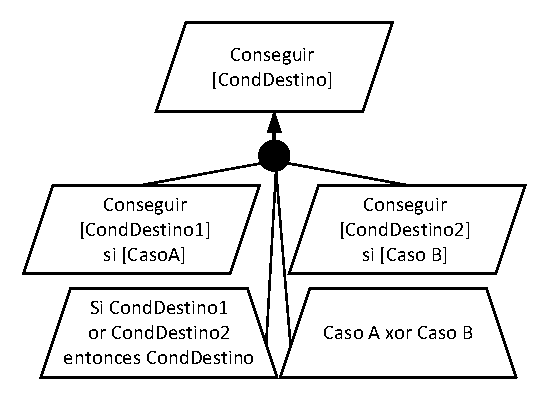
\includegraphics[width=0.70\linewidth,keepaspectratio=true]{images/objetivos/casePattern.eps}
    \end{center}
\end{frame}

\begin{frame}[c]
    \frametitle{Patrón Introducir Guarda}
    \begin{center}
        \includegraphics[width=0.70\linewidth,keepaspectratio=true]{images/objetivos/guardPattern.eps}
    \end{center}
\end{frame}

\begin{frame}[c]
    \frametitle{Patrón Divide y Vencerás}
    \begin{center}
        \includegraphics[width=0.70\linewidth,keepaspectratio=true]{images/objetivos/divideAndConquerPattern.eps}
    \end{center}
\end{frame}

\begin{frame}[c]
    \frametitle{Patrón Condición No Observable}
    \begin{center}
        \includegraphics[width=0.70\linewidth,keepaspectratio=true]{images/objetivos/unmonitorabilityPattern.eps}
    \end{center}
\end{frame}

\begin{frame}[c]
    \frametitle{Patrón Condición No Controlable}
    \begin{center}
        \includegraphics[width=0.70\linewidth,keepaspectratio=true]{images/objetivos/uncontrolabilityPattern.eps}
    \end{center}
\end{frame}

\section{Modelado y Especificación de Escenarios}

\subsection{Definición de Escenario}

\begin{frame}
    \frametitle{Proceso de Ingeniería de Requisitos}
	\rput[lt](0,-0.5){
	   \includegraphics[width=11.5cm,keepaspectratio=true]{images/escenarios.eps}}
\end{frame}

\begin{frame}[c]
    \frametitle{Definición de Escenario}
    \begin{block}{Escenario~\cite{pohl:2010}}
            Un \alert{\emph{escenario}} describe un ejemplo concreto de satisfacción, o fallo en la satisfacción, de un determinado objetivo o conjunto de objetivos.
    \end{block}
\end{frame}

\begin{frame}[c]
    \frametitle{Tipos de Escenarios}
    \begin{enumerate}[<+->]
        \item Sistema actual o sistema a construir.
        \item Positivos o negativos (permitidos o prohibidos).
        \item Descriptivos, exploratorios o explicativos.
        \item De tipos, de instancia o mixtos.
        \item Internos, de interacción con el sistema o de contexto.
        \item Principal, alternativo o excepcional.
    \end{enumerate}
\end{frame}

%\begin{frame}[t]
%    \frametitle{Escenarios de mal uso (misuse scenarios)}
%    \begin{block}{Escenarios de mal uso}
%        Un \emph{escenario de mal uso} documenta una secuencia de interacciones en las cuales un actor hostil intenta utilizar el sistema en contra de los objetivos de los \emph{stakeholders}.
%    \end{block}
%\end{frame}

%\begin{frame}[t]
%    \frametitle{Especificación de Escenarios}
%    \begin{block}{Escenarios de mal uso}
%        Un \emph{escenario de mal uso} documenta una secuencia de interacciones en las cuales un actor hostil intenta utilizar el sistema en contra de los objetivos de los \emph{stakeholders}.
%    \end{block}
%    %% TODO: Poner ejemplo
%\end{frame}

\begin{frame}[c]
    \frametitle{Escenario de Éxito, Escenario Principal y Extensión}
    \begin{description}[<+->]
        \item[Escenario de Éxito] Escenario que termina con la satisfacción del objetivo.
        \item[Escenario de No Éxito] Escenario que no es de éxito.
        \item[Escenario Principal] Escenario de éxito que describe el modo habitual de utilización del sistema.
        \item[Extensión] Fragmento de un escenario que describe una variación, de éxito o no, del mismo.
        \item[Condición de Extensión] Razones o circunstancias por las cuales un cierto comportamiento se desvía de su escenario principal y entra en una extensión.
    \end{description}
\end{frame}

\subsection{Elementos de un Escenario}

\begin{frame}[c]
    \frametitle{Elementos de un Escenario}
    \begin{description}[<+->]
        \item[Evento de Disparo (Trigger)] Evento que da lugar al inicio del caso de uso.
        \item[Precondición] Condición necesaria para que el escenario termine con éxito.
        \item[Garantías Mínimas] Condición mínima que ha de satisfacerse cuando el objetivo del escenario no puede alcanzarse.
        \item[Garantías de Éxito] Condición que se cumple siempre y cuando el escenario termina con éxito.
        \item[Paso] Acción con o del sistema que puede ser:
             \begin{small}
             \begin{enumerate}[<+->]
                 \item Una interacción entre un actor y el sistema (en cualquier dirección);
                 \item Una validación para proteger algún objetivo de un \emph{stakeholder};
                 \item Un cambio interno en el sistema para satisfacer algún objetivo de un \emph{stakeholder}.
            \end{enumerate}
            \end{small}
        \item[Escenario Principal] Conjunto de pasos que describen el escenario principal.
        \item[Extensiones] Descripción de las posibles extensiones.
    \end{description}
\end{frame}

\subsection{Reglas de Escritura de Escenarios}

\begin{frame}[c]
    \frametitle{Reglas de Escritura de Escenarios}
    \begin{enumerate}[<+->]
        \item Usar una gramática simple.
        \item Indicar claramente quién tiene el control y quién recibe resultado de las acciones.
        \item Escribir el caso de uso \emph{desde fuera del sistema}.
        \item Mostrar el proceso avanzando.
        \item Describir las intenciones del usuario, no sus movimientos.
        \item Escribir \emph{validar}, en lugar de \emph{el sistema comprueba si}.
        \item Mencionar si es necesario la temporización.
        \item Escribir \emph{el usuario require que el sistema ...} para acciones con terceros.
        \item Truco: \emph{Repetir los pasos X-Y hasta que $<$condición$>$}.
        \item Truco: \emph{Los pasos X-Y pueden suceder en cualquier orden}.
    \end{enumerate}
\end{frame}

\begin{frame}[c]
    \frametitle{Identificación de Extensiones}
    \begin{enumerate}[<+->]
        \item Identificar, mediante una técnica adecuada, todas las desviaciones del escenario principal que se consigan imaginar. Prestar atención a:
            \begin{enumerate}
                \item Caminos de éxito alternativos.
                \item Comportamientos erróneos del actor primario y último.
                \item Inactividad del actor primario y último.
                \item Inactividad de un actor secundario con el que interactua el sistema.
                \item Caminos alternativos para \emph{el sistema valida}.
                \item Fallo interno, detectable y recuperable del sistema.
                \item Fallos inesperados.
                \item Fallos de rendimiento.
            \end{enumerate}
        \item Descartar aquellas extensiones cuyas condiciones sean indetectables.
        \item Fusionar aquellas extensiones cuyas condiciones y efecto sean equivalente.
        \item Escribir cada extensión.
    \end{enumerate}
\end{frame}

\begin{frame}[c]
    \frametitle{Formas de Terminación de una Extensión}
    \begin{enumerate}[<+->]
        \item El caso de uso sigue un camino de éxito alternativo.
        \item La situación anómala se soluciona y el caso de uso prosigue normal.
        \item Se da al usuario una nueva oportunidad y el caso de uso prosigue normal.
        \item Se detecta un fallo insalvable y el caso de uso termina.
     \end{enumerate}
\end{frame}

\begin{frame}[c]
    \frametitle{Reglas de Escritura de Extensiones}
    \begin{enumerate}[<+->]
        \item Hacer que la condición exprese \alert{\emph{qué}} se ha detectado.
        \item Identar el cuerpo de la extensión.
    \end{enumerate}
\end{frame}

\section{Historias de Usuario}

\begin{frame}[c]
	\frametitle{Historia de Usuario (\emph{User Story})}
	\begin{block}{Historia de Usuario}
        Un \emph{historia de usuario} describe una funcionalidad del sistema que posee valor para algún \emph{stakeholder} del sistema.
        \uncover<2->{Una historia de usuario se compone de tres elementos:
        \begin{description}
            \item<3->[Tarjeta] Cada historia de usuario se anota en una tarjeta física, que representa la historia de usuario.
            \item<4->[Conversación] Corresponde con las conversaciones (efímeras) mantenidas entre las diferentes personas involucradas en el desarrollo de la historia de usuario, tales como usuarios, clientes, testadores, programadores, etc. Se puede documentar parte de estas conversaciones.
            \item<5->[Confirmación] Procedimiento para verificar que la historia de usuario ha sido realizada.
        \end{description}
        }
	\end{block}
\end{frame}

\begin{frame}[c]
	\frametitle{Propiedades Deseables de una Historia de Usuario}
	\begin{enumerate}[<+->]
		\item Independiente.
        \item Abierta.
        \item De valor para algún stakeholder.
        \item Estimable.
        \item Pequeñas.
        \item Verificable (testable).
	\end{enumerate}
\end{frame}

\begin{frame}[c]
	\frametitle{Historia Épica}
	\begin{block}{Historia Épica}
        Una historia épica (\emph{epic}) es una historia que por su tamaño no puede ser desarrollada en un periodo corto de tiempo (15 días), por lo que ha de ser descompuesta en historias de usuario de menor tamaño.
	\end{block}
\end{frame}

\section{Sumario y Referencias}

\subsection{Sumario}

\begin{frame}[c]
    \frametitle{¿Qué Tengo que Saber de Todo Esto?}
    \begin{enumerate}[<+->]
        \item Saber identificar, estructurar y especificar requisitos a diferentes niveles de abstracción.
        \item Ser capaz de construir modelos orientados a objetivos utilizando los lenguajes KAOS y/o GRL.
        \item Ser capaz de especificar escenarios de forma completa, incluyendo extensiones.
        \item Ser capaz de especificar requisitos como historias de usuario.
        \item Comprender el papel de los modelos orientados a la solución en Ingeniería de Requisitos y cómo se elaboran.
    \end{enumerate}
\end{frame}

\subsection{Referencias}
%
\begin{frame}
	\frametitle{Referencias}
	%\nocite{cockburn:2000,pohl:2010,lamsweerde:2009,itu:urn,Cohn2004}
	\bibliographystyle{apalike}
	\bibliography{ir}
\end{frame}

\end{document}
